\Chapter{Szimuláció}

\Section{Megvalósítása}

Ahhoz, hogy kezelni tudjam a győzelmet befolyásoló tényezőket, szükségem volt egy olyan programrészre, mely képes gépi játékosokkal sokszor lejátszani egy-egy játékot, mert a nagy számok törvénye alapján statisztikailag kimutatható, hogy a szerencsének alacsony a befolyása magasabb játékszám esetén.

	Alapját az emberi játékosok által is játszható kódok alkotják, így a szerver részét alakítottam át úgy, hogy alkalmas legyen az általam megadott paraméterek vizsgálatára. Az összes szimulációt a simulations nevű mappában tárolom külön fájlokban, hogyha később újra megkell vizsgálnom őket, egymástól függetlenül is teljes értékű eredményeket biztosítsanak.  A játékok egymás utáni többszöri lejátszásának egy for ciklus biztosít lehetőséget.

\begin{javascript}
for(var g=0; g<turns;g++){
  botGame();
  if(game.rounds<roundLimit){
    full_turns++;
    changeRanks();
  }
}
\end{javascript}


Előre inicializáltam a turns, roundLimit illetve full\_turns változókat, a szimulációk könnyebben kezelhetőségéért. A turns-el állítható be a lefuttatni kívánt játékok mennyisége. Annak érdekében, hogy valós értékeken belül maradjunk, megszabtam  egy maximális kört a játékok számára, ennek értékét a roundLimit tárolja. A full\_turns pedig a statisztikai adatok kinyerésében fog a későbbiekben fontosabb szerepet játszani, hiszen hiába futtattunk például 10000 játékot, ha abból csak 9995 volt a megszabott határon belül. Ennek függvényében nyilvánvalóan pontosabb adatokat fogunk kinyerni a szimulációból és ezáltal a méréseink is hitelesebbek lesznek.


\Section{Paraméterek randomizálása}

Az értékek megadását tapasztalatokra, illetve megismert stratégiákra alapoztam. Nem akartam a valóságtól elrugaszkodott túlzottan alacsony, illetve magas értékekkel dolgozni, hiszen az nem adná vissza számunkra egy játék valós kimenetelét. Paraméterértékek zárt intervallumai, illetve az utolsó két érték százalékos esélye:

\begin{itemize}
	\item tradeRate: 1.2 - 2.5
	\item tradeIncrement: 0.2 - 2.1
	\item maxRejectCount: 3 - 10
	\item maxUpgradeCount: 3 - 5
	\item minMoneyAfterTrade: 0 - 40000
	\item minMoneyAfterBuy: 0 - 40000
	\item stayInJailRound: 20 - 50
	\item needBusiness: 50\%
	\item needService: 50\%
\end{itemize}

\Section{Átlagos körhossz}

Első tesztelésem során azt vizsgáltam, hogy egy játék alatt hány kör zajlik le. Egy egész körnek az számít, hogyha az összes, még játékban lévő játékos dobott egymás után, és újra az következik akinél kezdődtek a dobások. Mind a négy botnak véletlenszerű paramétereket állítottam be, hogy azonos esélyekkel induljanak, és ez ne befolyásolja nagy mértékben a kapott értékeket.

A szimulációt 100000 játékra állítottam, ezt az értéket kellően elégnek gondolom az átlag megállapításához. Létrehoztam egy avg\_rounds számlálót, ami minden lejátszott kör után, mely a határértéken belül volt, nő a kör számával. Az összes játék végét követően elosztom a full\_turns változóval. Közben vizsgálom, hogy mennyi azonos kör volt a játékok során.  Az átlagos körhossz 36,9 volt.

Az előző adatokat \aref{fig:korok}. ábrán látható grafikon segítségével szemléltetem.

\begin{figure}[h!]
\centering
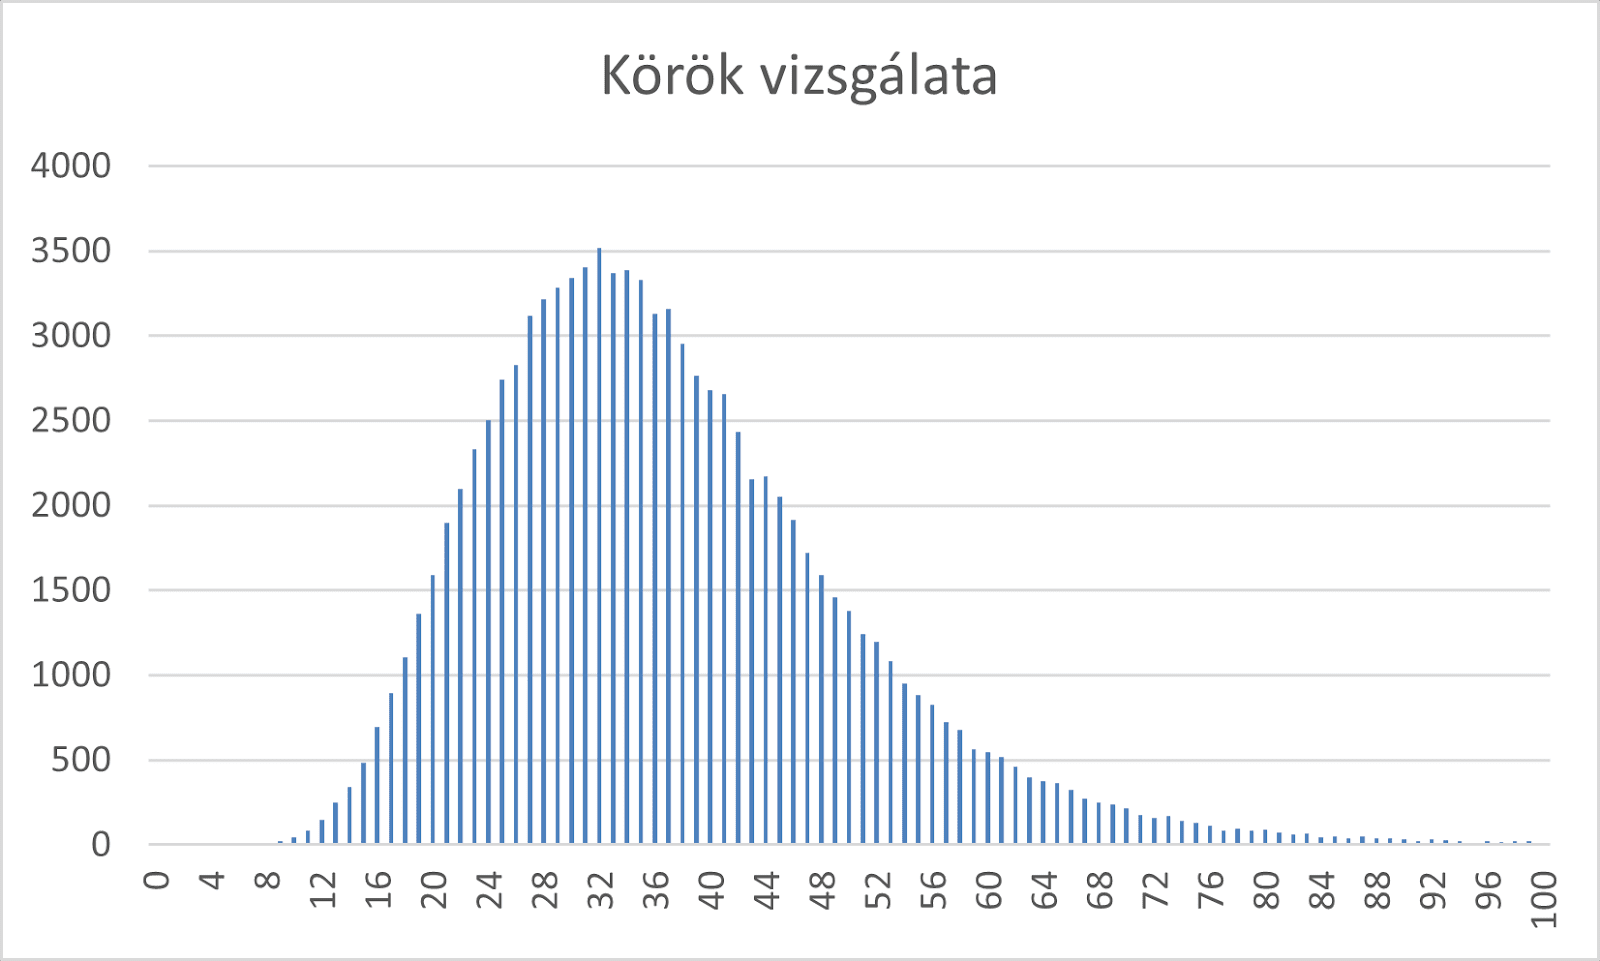
\includegraphics[scale=0.2]{images/Kep1.png}
\caption{Körök vizsgálata}
\label{fig:korok}
\end{figure}

\Section{Paraméterek optimalizálása}

A következőkben a legoptimálisabb paramétereket fogom megkeresni, amelyek alapján a kiválasztott botunk a lehető legjobb eredményeket tudja produkálni. Először általunk jónak vélt paraméterezéssel látjuk el a botot melyet vizsgálni fogunk. Majd a paramétereket egyesével egymás után váltjuk le a mérések során kapott legjobb értékekre. A futtatások száma paraméteren értékekként 100000 lesz.

\begin{itemize}
	\item tradeIncrement: 0.3
	\item maxRejectCount: 5
	\item maxUpgradeCount: 5
	\item minMoneyAfterTrade: 0
	\item minMoneyAfterBuy: 0
	\item stayInJailRound: 20
	\item needBusiness: true
	\item needService: true
\end{itemize}

\begin{javascript}
function giveParameters(p){
  var p1_parameters={
    name: 'Elso',
    tradeRate: p,
      ...
  }
  ...
}
\end{javascript}

Szükségem volt egy külső ciklusra, a már megírt játékok futtatása köré, mely folyamatosan változtatja a kiválasztott botunk éppen vizsgált paraméterét. Példánkban a tradeRate paramétert vizsgáltam. Ezt az értéket nem reális 2.5 érték felé vinni, ezért ez a maximum.
\newpage
\subsection{tradeRate}
Lépésköz: 0.1
\begin{figure}[h!]
\centering
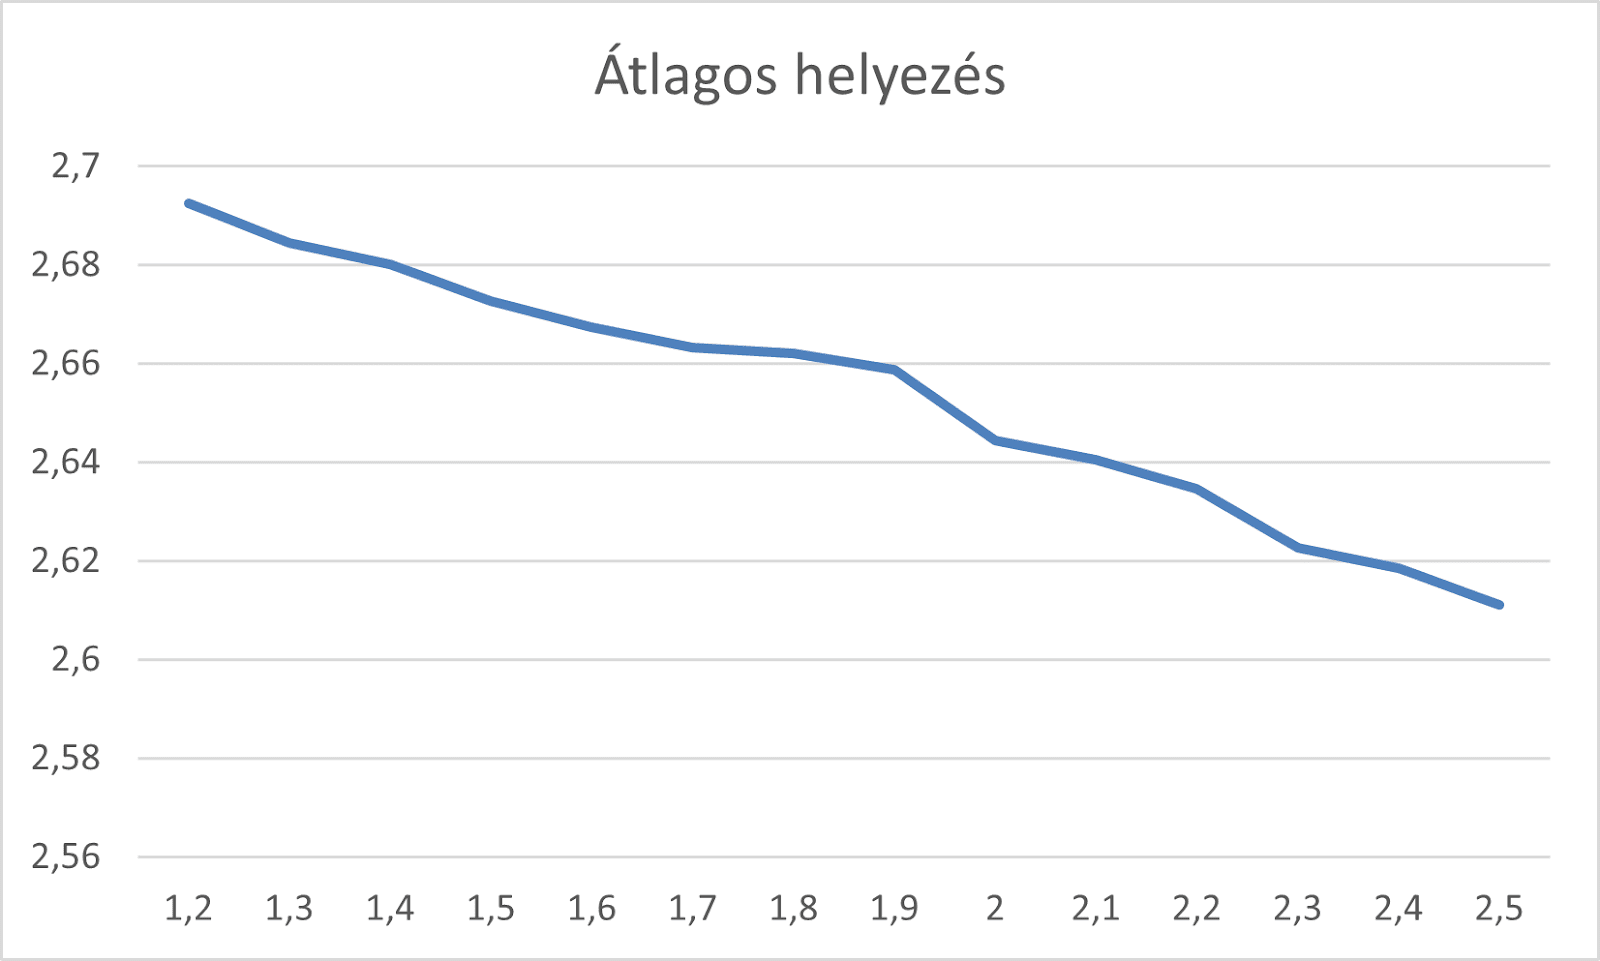
\includegraphics[scale=0.2]{images/Kep1w.png}
\caption{tradeRate vizsgálata}
\label{fig:ff}
\end{figure}

Az adott intervallumon való vizsgálat során a 2.5-ös paraméter volt a legjobb.

\subsection{tradeIncrement}
Lépésköz: 0.1
\begin{figure}[h!]
\centering
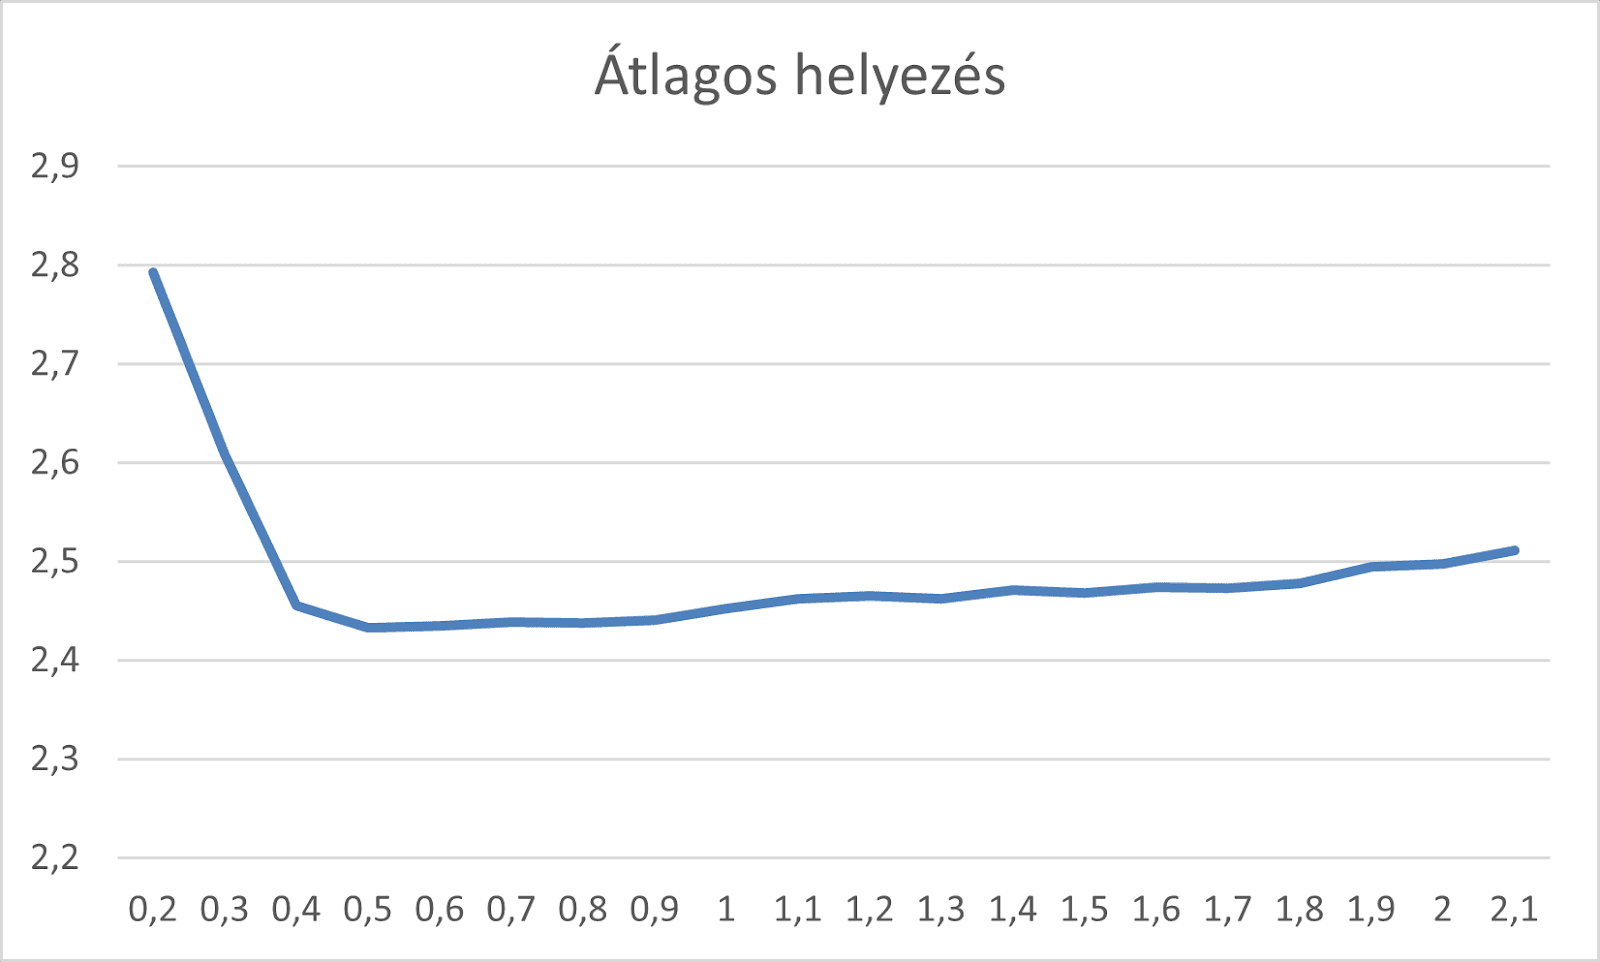
\includegraphics[scale=0.2]{images/sdf.png}
\caption{tradeIncrement vizsgálata}
\label{fig:ff}
\end{figure}

Amint az ábrán is láthatjuk, a függvény minimuma a 0.5-ös paraméternél helyezkedik el.
\newpage

\subsection{maxRejectCount}
Lépésköz: 1
\begin{figure}[h!]
\centering
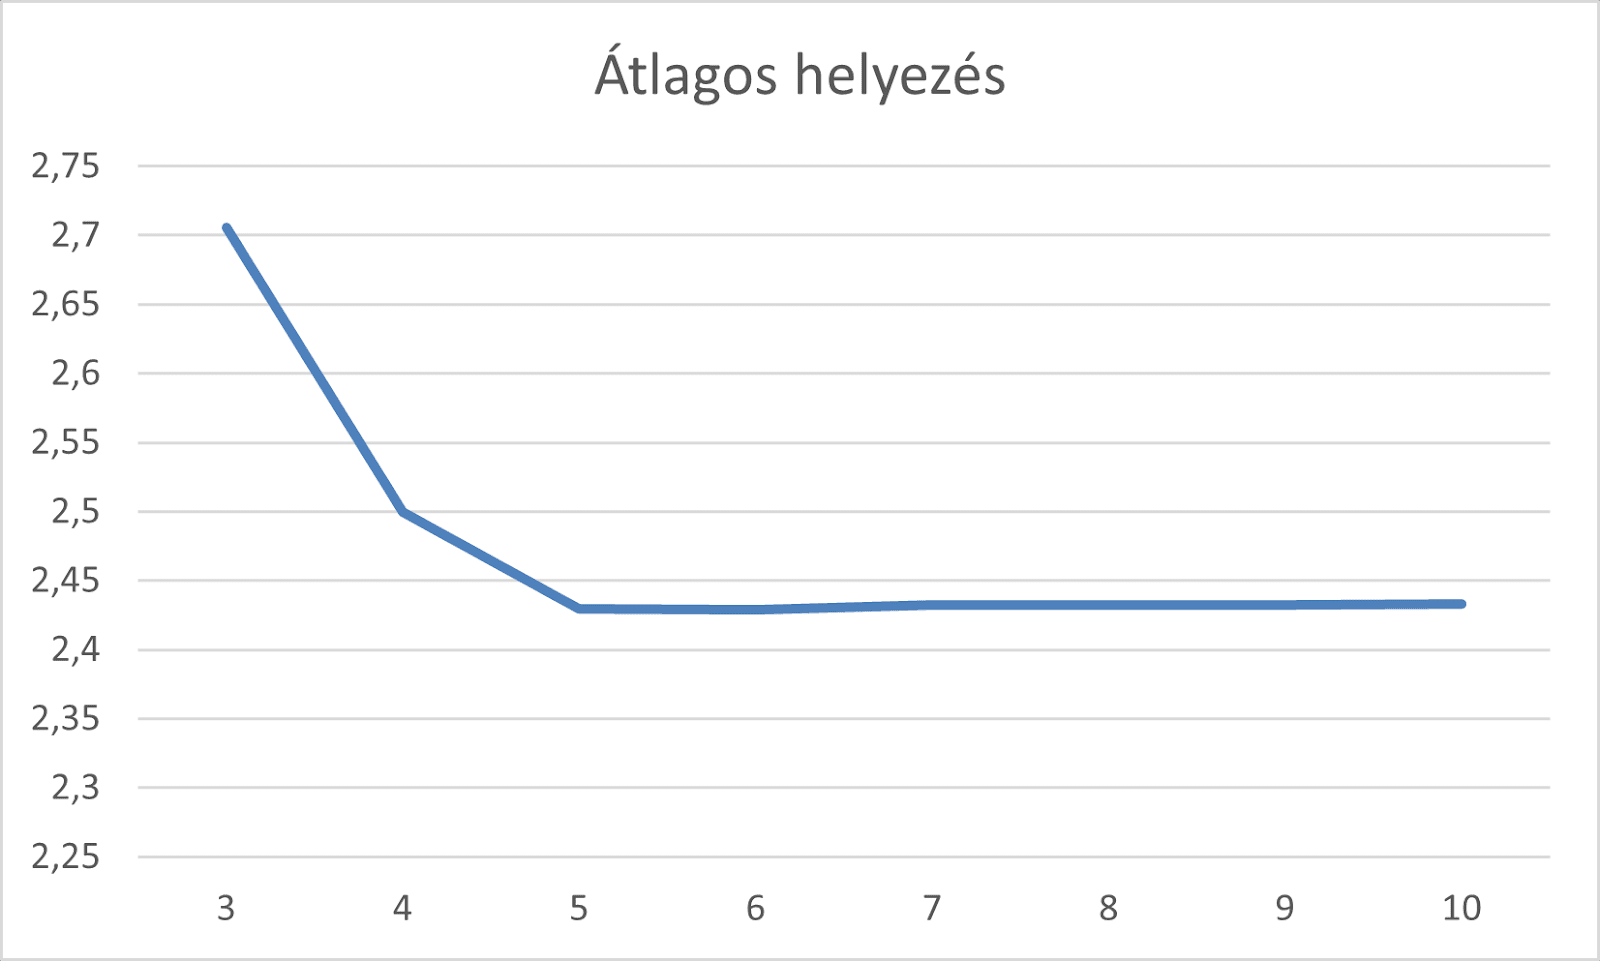
\includegraphics[scale=0.2]{images/ff.png}
\caption{maxRejectCount vizsgálata}
\label{fig:ff}
\end{figure}

A függvényből megállapíthatjuk, hogy a 6-os paramétertől felfelé egy lassú növekvő monotonitás érzékelhető, így ezt az értéket tekintjük a vizsgálat szempontjából a legmegfelelőbbnek.

\subsection{maxUpgradeCount}
Lépésköz: 1
\begin{figure}[h!]
\centering
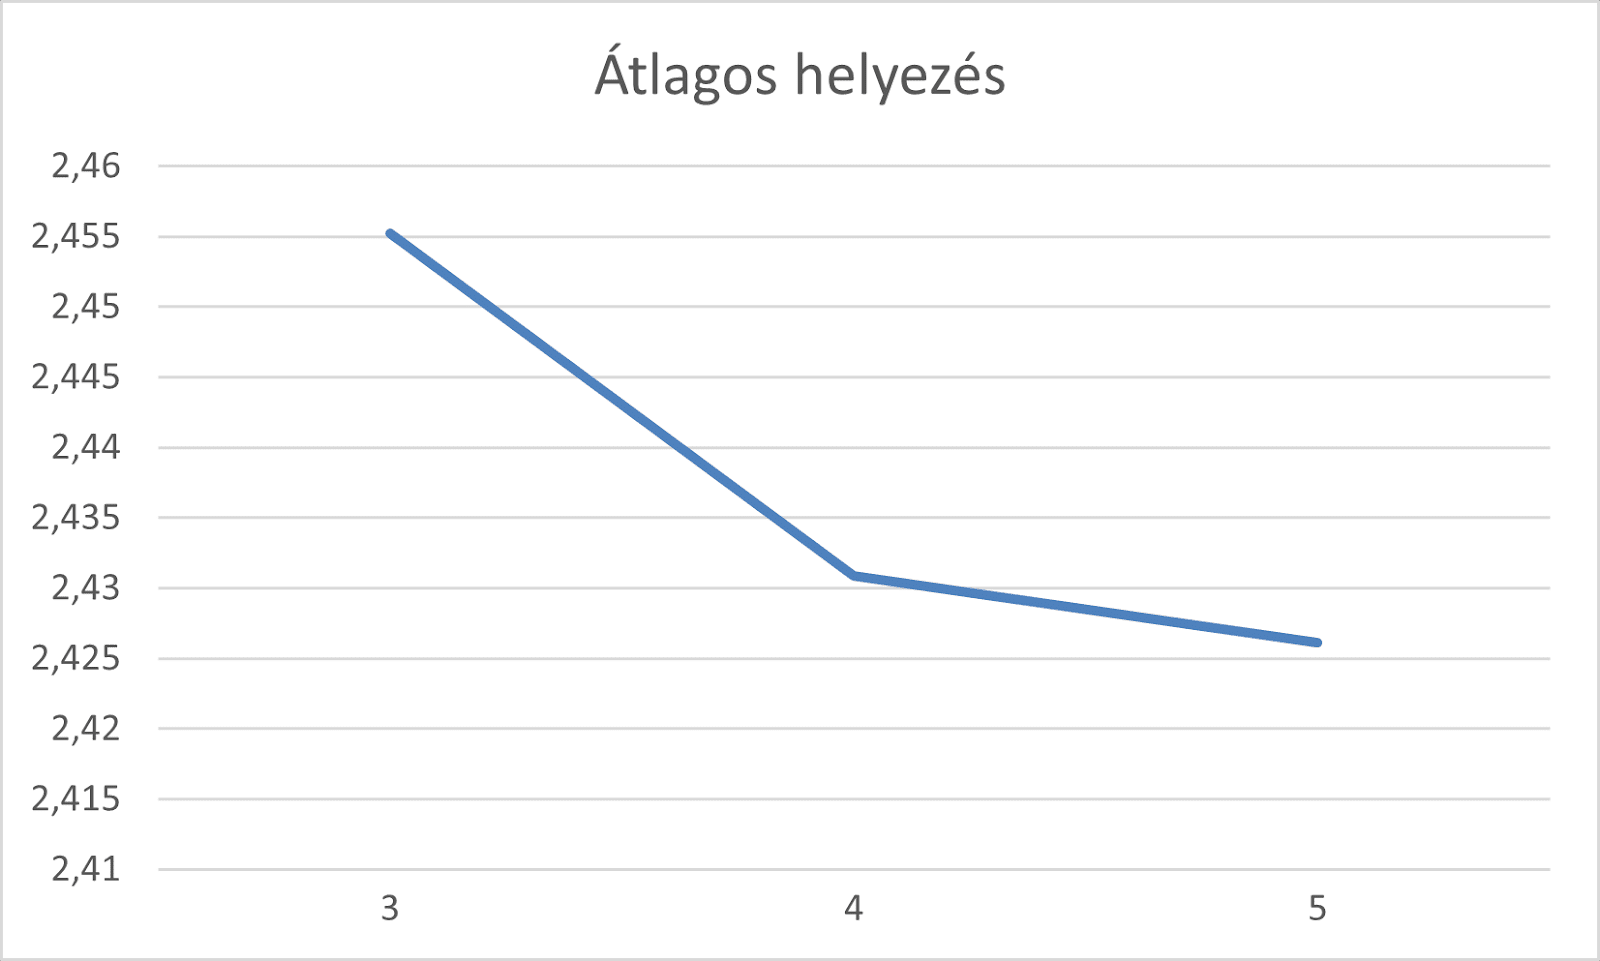
\includegraphics[scale=0.2]{images/bbb.png}
\caption{maxUpgradeCount vizsgálata}
\label{fig:ff}
\end{figure}

Legjobb eredmény:  2,432351 a 0.5-ös paramétert használva.
\newpage
\subsection{minMoneyAfterTrade}
Lépésköz: 1000
\begin{figure}[h!]
\centering
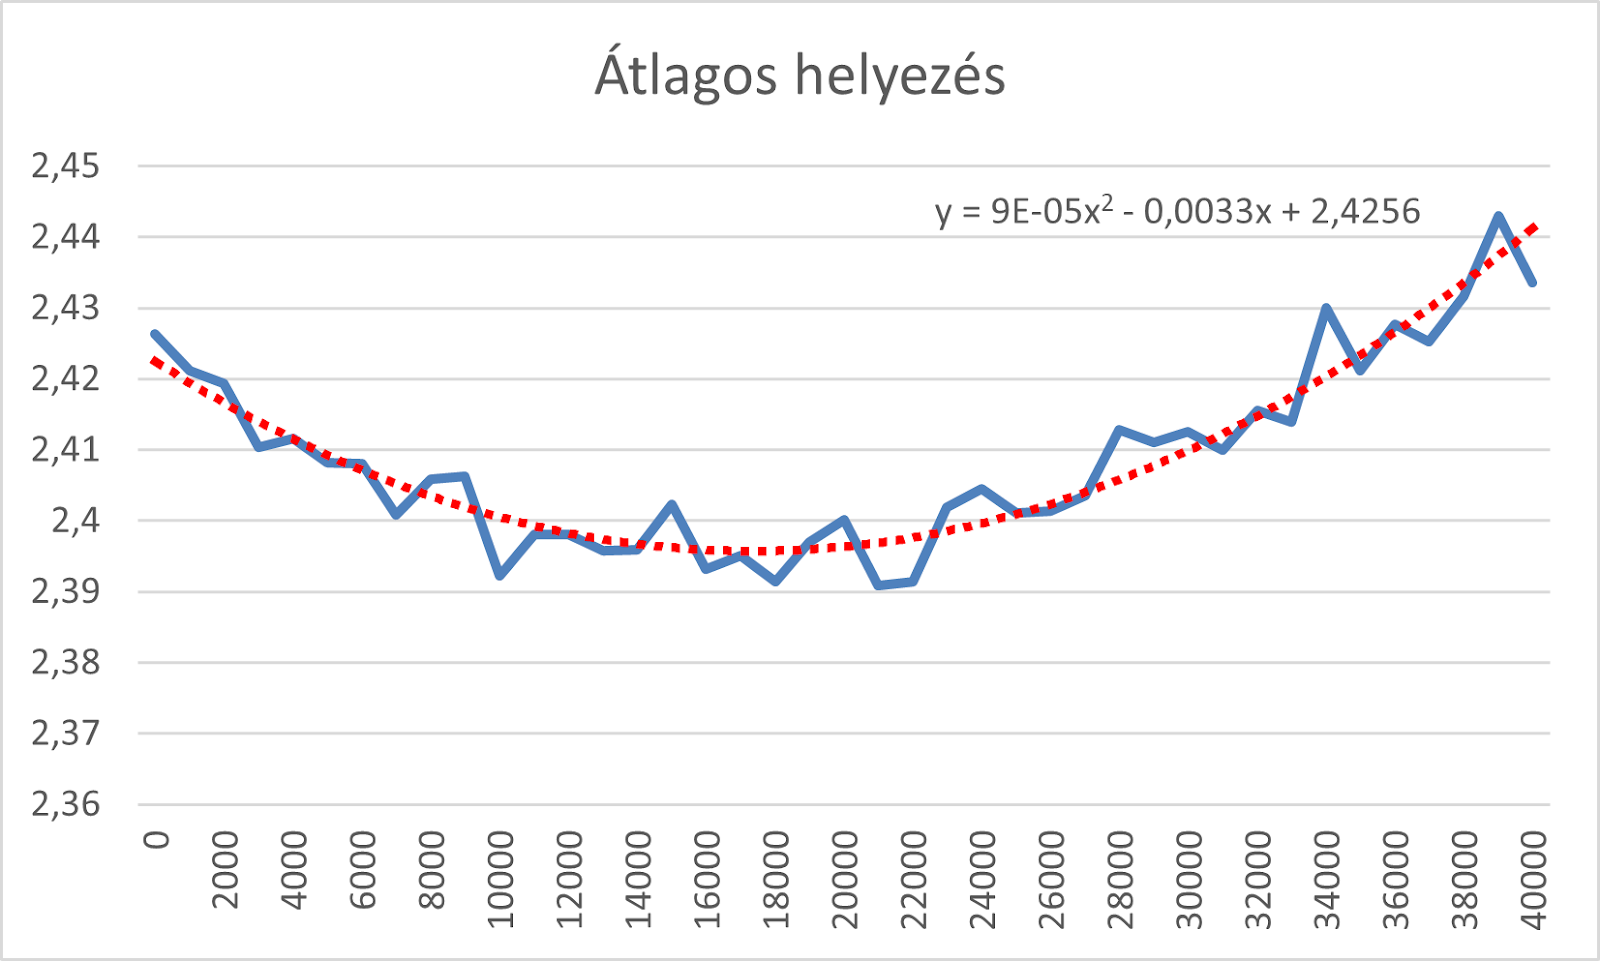
\includegraphics[scale=0.2]{images/aaaaaaaaa.png}
\caption{minMoneyAfterTrade vizsgálata}
\label{fig:ff}
\end{figure}

Zajos függvényt kaptuk, de megállapítható, hogy körülbelül a 10000-22000 intervallumon belül érdemes maradni.

\subsection{minMoneyAfterBuy}
Lépésköz: 1000
\begin{figure}[h!]
\centering
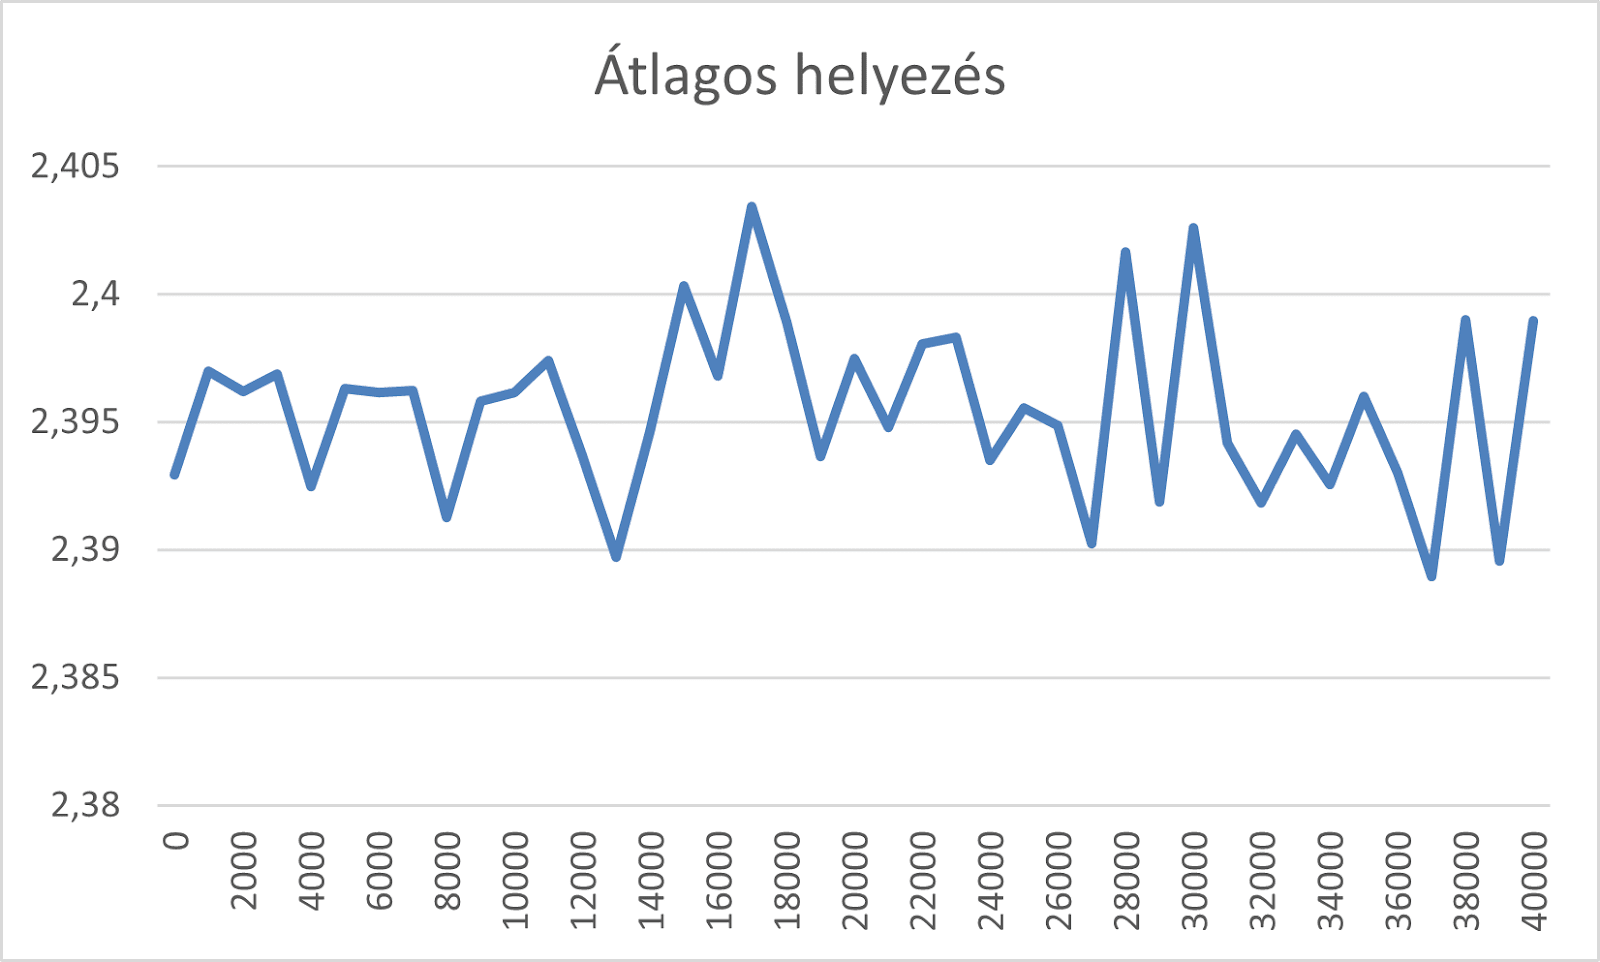
\includegraphics[scale=0.2]{images/fdgd.png}
\caption{minMoneyAfterBuy vizsgálata}
\label{fig:ff}
\end{figure}

Túlságosan zajos képet kaptam, ezért nem állapítható meg következtetés.
\newpage
\subsection{stayInJailRound}
Lépésköz: 1
\begin{figure}[h!]
\centering
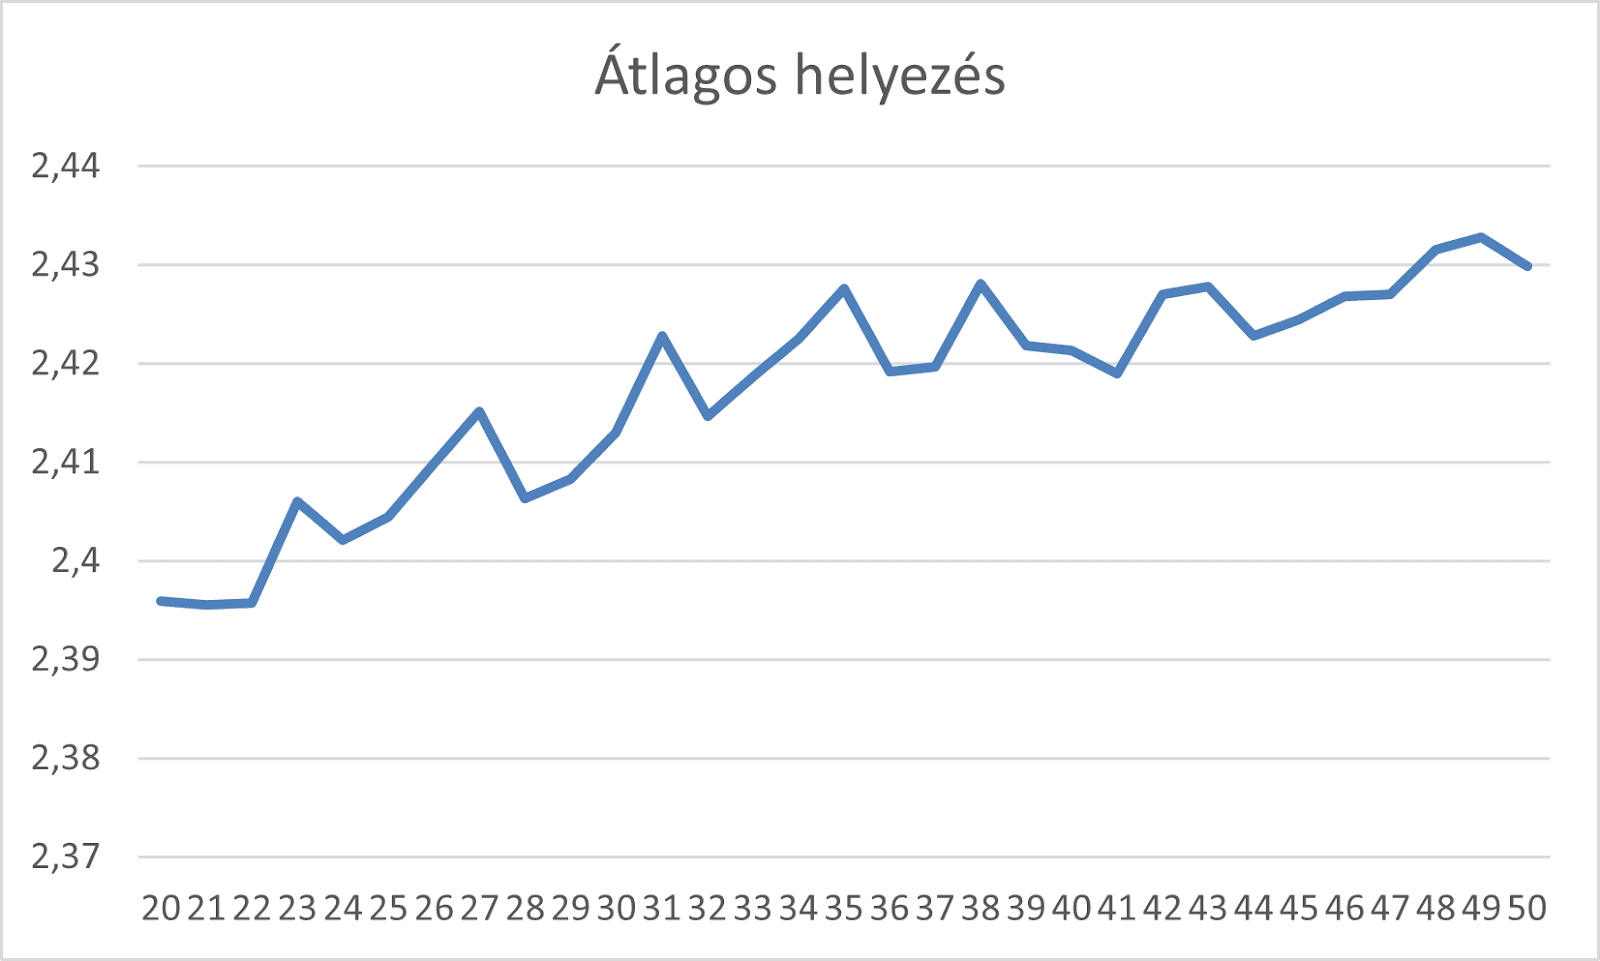
\includegraphics[scale=0.2]{images/dfg.png}
\caption{stayInJailRound vizsgálata}
\label{fig:ff}
\end{figure}

Jól szemlélteti a függvény, hogy a 21-es paraméter használata után egyre drasztikusabb eredményeket produkál.

\subsection{needBusiness}
Lépésköz: 1
\begin{figure}[h!]
\centering
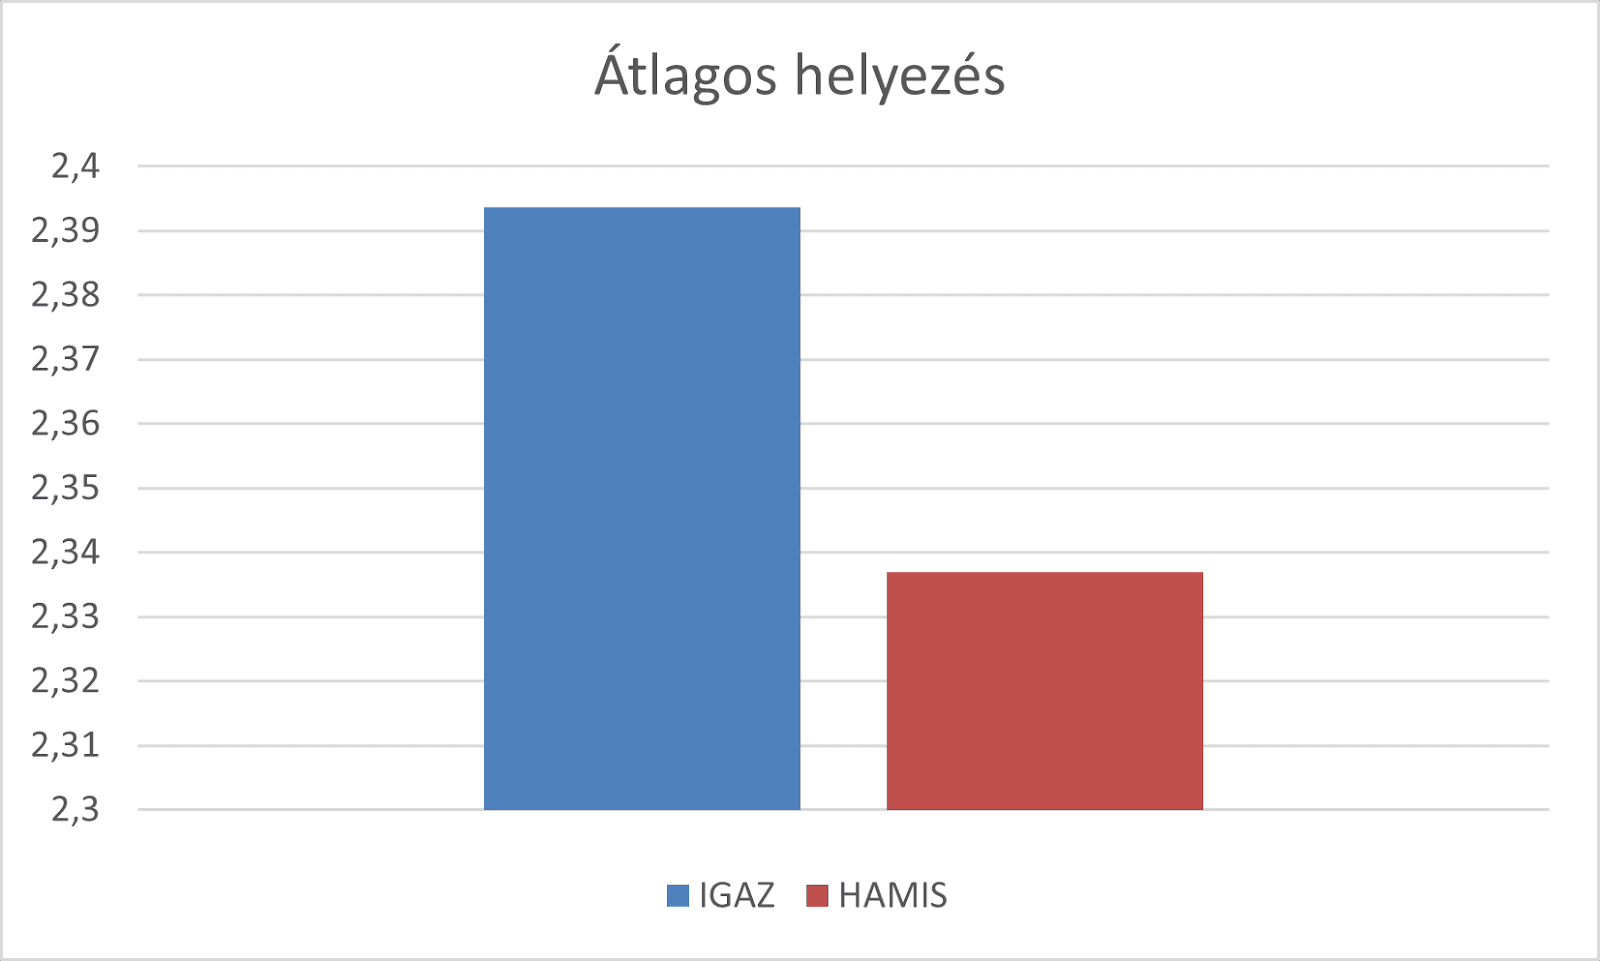
\includegraphics[scale=0.2]{images/bbbbbb.png}
\caption{needBusiness vizsgálata}
\label{fig:ff}
\end{figure}

A false paraméter értéket választva a kapott eredményünk 2,33687.
\newpage
\subsection{needService}
Lépésköz: 1
\begin{figure}[h!]
\centering
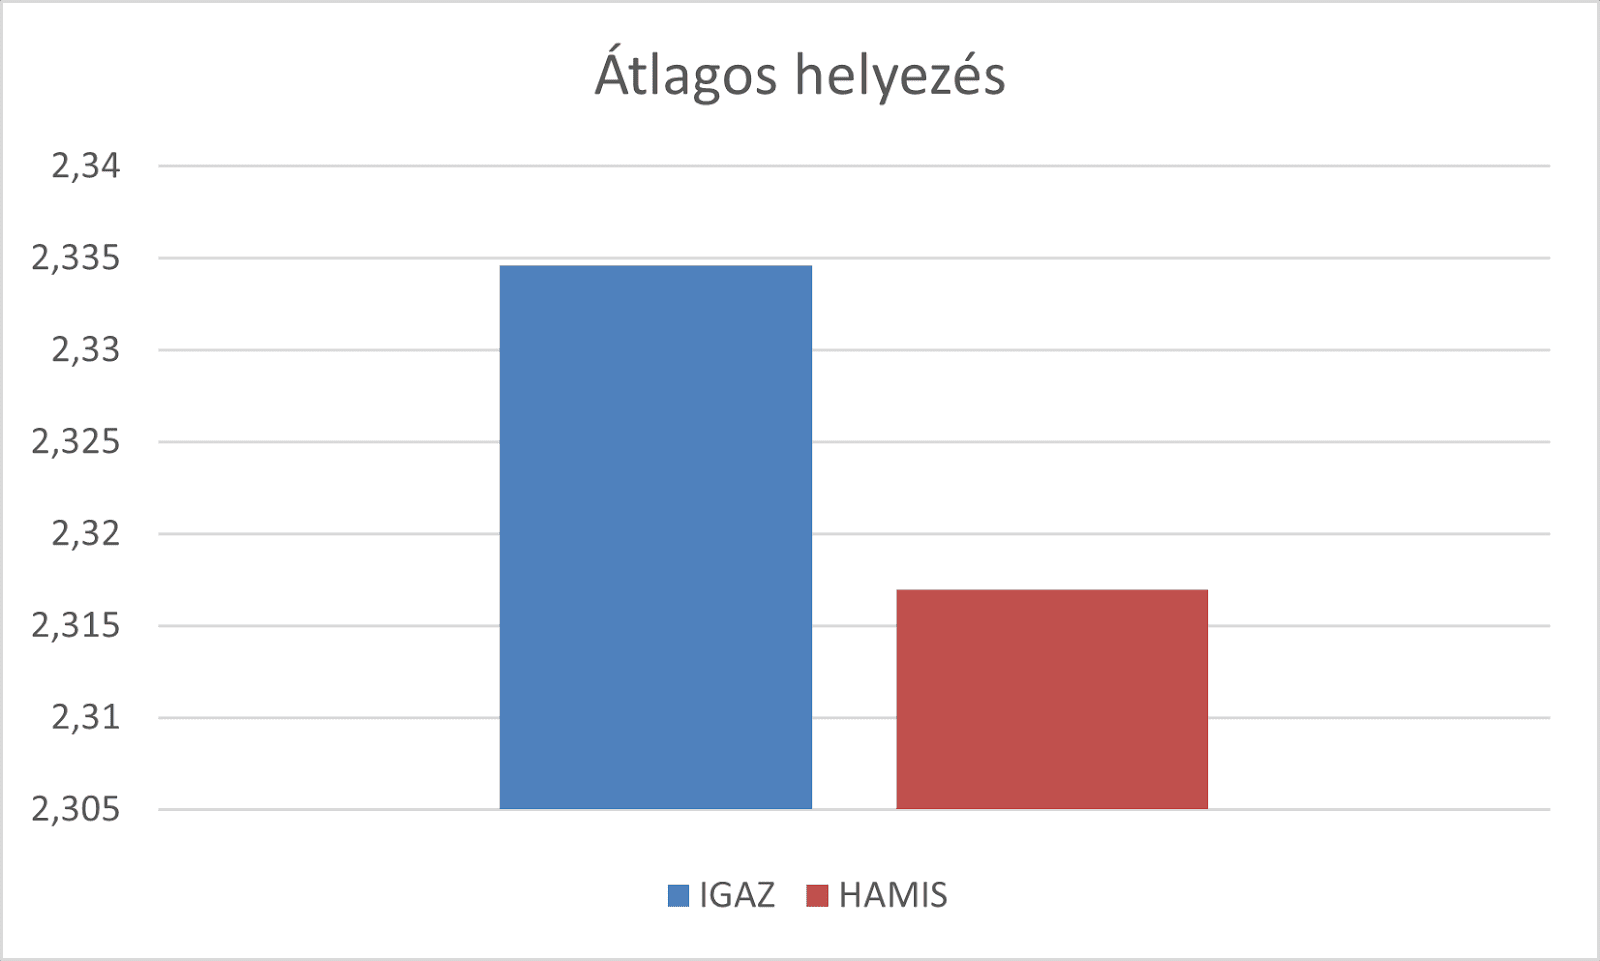
\includegraphics[scale=0.2]{images/ccvv.png}
\caption{needService vizsgálata}
\label{fig:ff}
\end{figure}

A false paraméter értéket választva a kapott eredményünk 2,316989.